\documentclass[11pt,a4paper]{article}

\usepackage[utf8]{inputenc}
\usepackage[T1]{fontenc}
\usepackage{lmodern}
\usepackage[margin=2.5cm]{geometry}
\usepackage{amsmath,amssymb}
\usepackage{graphicx}
\usepackage{booktabs}
\usepackage{adjustbox}
\usepackage{float}
\usepackage{caption}
\usepackage[hidelinks]{hyperref}

\graphicspath{{../outputs/figures/}}
\captionsetup{font=small,labelfont=bf}
\setlength{\parskip}{0.5em}
\setlength{\parindent}{0pt}

\newcommand{\E}{\mathbb{E}}
\newcommand{\N}{\mathcal{N}}

\title{\textbf{European Option Pricing:\\ Comparison of Binomial Trees and the Black--Scholes Model}\\[0.5em]
\large MAC F244 --- Project Report}
\author{}
\date{November 2026}

\begin{document}
\maketitle

\begin{center}
\begin{tabular}{ll}
\toprule
\textbf{Name} & \textbf{ID No.} \\
\midrule
Mohammad Zaid Agha & 2024ADPS0840G \\
Adwait Eklavya & 2024ADPS0825G \\
Shivank Mishra & 2024ADPS0823G \\
Aswin Sunderiyal & 2024ADPS0867G \\
Rayasam Venkata Pradyumn & 2024B5AD0973G \\
\bottomrule
\end{tabular}
\end{center}

\begin{abstract}
We price European call and put options on three NSE-listed stocks with two methods: the closed-form Black--Scholes (BS) formula and the Cox--Ross--Rubinstein (CRR) binomial tree. Volatility is estimated from one year of daily prices and the risk-free rate is taken from the RBI 364-day Treasury Bill yield. We show that the binomial price converges to the BS price as the number of steps $n$ grows, with an error that falls like $1/n$ and a sign that alternates between odd and even $n$. We study how strike, volatility, maturity and the choice of stock affect the prices and the gap between the two models, and we compare running times. At $n = 500$ the binomial price is within about $0.04\%$ of the BS price for an at-the-money call on every stock tested, while the BS formula is roughly $34$ times cheaper than a $1000$-step tree.
\end{abstract}

\tableofcontents
\newpage

%% ------------------------------------------------------------------
\section{Introduction}

A \emph{European option} gives its holder the right, but not the obligation, to buy (call) or sell (put) an asset at a fixed strike price $K$ on a fixed future date $T$. If $S_T$ is the stock price at that date, the payoff is $\max(S_T - K, 0)$ for a call and $\max(K - S_T, 0)$ for a put. The question is what the option should cost today.

Two standard answers are used in practice and in teaching:
\begin{itemize}
  \item the \textbf{Black--Scholes model} \cite{blackscholes1973}, in which the stock price moves continuously and the option price is given by an explicit formula;
  \item the \textbf{binomial tree model} of Cox, Ross and Rubinstein \cite{crr1979}, in which time is cut into $n$ small steps and the stock can only move up or down at each step; the price is found by working backwards through the tree.
\end{itemize}
The binomial model is built to approximate the Black--Scholes model, so the two should agree when $n$ is large. In this project we price the same options with both methods and measure how close they get, how fast, and at what computational cost.

\textbf{Objectives.}
\begin{enumerate}
  \item Implement both models in Python and verify them against known values.
  \item Show how the binomial price approaches the BS price as $n$ increases, and measure the rate.
  \item Study how strike, volatility, maturity and the stock itself change the prices and the discrepancy.
  \item Compare the running time of the two methods.
\end{enumerate}

\textbf{Outline.} Section~\ref{sec:model} gives the mathematics, Section~\ref{sec:data} the data and parameters, Section~\ref{sec:impl} the implementation and its verification, Section~\ref{sec:results} the results, and Sections~\ref{sec:discussion}--\ref{sec:conclusion} the discussion, limitations and conclusions.

%% ------------------------------------------------------------------
\section{Mathematical model}\label{sec:model}

\subsection{Stock price model}

We assume the stock price follows geometric Brownian motion (GBM). Under the risk-neutral measure,
\begin{equation}\label{eq:gbm}
  dS = rS\,dt + \sigma S\,dW,
\end{equation}
where $r$ is the (continuously compounded) risk-free rate, $\sigma$ is the annualised volatility and $W$ is a standard Brownian motion. Equation~\eqref{eq:gbm} has the solution
\begin{equation}\label{eq:gbm-sol}
  S_T = S_0 \exp\!\Big(\big(r - \tfrac{1}{2}\sigma^2\big)T + \sigma W_T\Big),
\end{equation}
so $\ln(S_T/S_0)$ is normal with mean $(r - \sigma^2/2)T$ and variance $\sigma^2 T$. The price of a European option is its discounted expected payoff under this measure, for example $C = e^{-rT}\,\E[\max(S_T - K, 0)]$ for a call.

\subsection{The Black--Scholes formula}

Evaluating the expectation for the call with the log-normal law above gives the Black--Scholes formula \cite{blackscholes1973,hull}:
\begin{align}
  C &= S_0\,N(d_1) - K e^{-rT} N(d_2), \label{eq:bs-call}\\
  d_1 &= \frac{\ln(S_0/K) + (r + \sigma^2/2)\,T}{\sigma\sqrt{T}}, \qquad
  d_2 = d_1 - \sigma\sqrt{T}, \label{eq:d1d2}
\end{align}
where $N(\cdot)$ is the standard normal distribution function. The put price follows from put--call parity,
\begin{equation}\label{eq:parity}
  C - P = S_0 - K e^{-rT} \quad\Longrightarrow\quad P = C - S_0 + K e^{-rT}.
\end{equation}

\subsection{The Cox--Ross--Rubinstein binomial tree}

Divide $[0,T]$ into $n$ steps of length $\Delta t = T/n$. At each step the stock moves up by a factor $u$ or down by a factor $d$:
\begin{equation}\label{eq:crr}
  u = e^{\sigma\sqrt{\Delta t}}, \qquad d = \frac{1}{u}, \qquad
  p = \frac{e^{r\Delta t} - d}{u - d}.
\end{equation}
The probability $p$ is chosen so that the expected one-step growth equals the risk-free growth, $p\,u + (1-p)\,d = e^{r\Delta t}$. The choice $d = 1/u$ makes the tree \emph{recombining}: an up move followed by a down move returns to the starting price, so after $i$ steps there are only $i+1$ distinct prices rather than $2^i$. After $n$ steps with $j$ up moves the stock price is
\[
  S_{n,j} = S_0\, u^{j} d^{\,n-j} = S_0\, u^{\,2j-n}, \qquad j = 0,1,\dots,n.
\]
Let $V_{i,j}$ be the option value at step $i$ with $j$ up moves. At maturity it equals the payoff,
\[
  V_{n,j} = \max(S_{n,j} - K, 0) \quad\text{(call)}, \qquad V_{n,j} = \max(K - S_{n,j}, 0) \quad\text{(put)},
\]
and earlier values are found by discounted risk-neutral averaging,
\begin{equation}\label{eq:backward}
  V_{i,j} = e^{-r\Delta t}\big[\,p\,V_{i+1,j+1} + (1-p)\,V_{i+1,j}\,\big], \qquad i = n-1, \dots, 0.
\end{equation}
The option price is $V_{0,0}$. Unrolling the recursion gives the equivalent closed sum
\begin{equation}\label{eq:binom-sum}
  V_{0,0} = e^{-rT}\sum_{j=0}^{n} \binom{n}{j} p^{\,j} (1-p)^{n-j}\, V_{n,j}.
\end{equation}

\subsection{Why the binomial price converges to Black--Scholes}\label{sec:why}

After $n$ steps, $\ln(S_T/S_0) = \sigma\sqrt{\Delta t}\,(2J - n)$ where $J \sim \mathrm{Binomial}(n,p)$. For small $\Delta t$ the probability $p$ is close to $1/2$, with $p - \tfrac12 \approx \frac{(r-\sigma^2/2)}{2\sigma}\sqrt{\Delta t}$. To first order in $\Delta t$ this gives
\[
  \E\big[\ln(S_T/S_0)\big] \to \big(r - \tfrac12\sigma^2\big)T, \qquad
  \mathrm{Var}\big[\ln(S_T/S_0)\big] \to \sigma^2 T,
\]
which are exactly the mean and variance in \eqref{eq:gbm-sol}. By the central limit theorem the binomial distribution of $\ln(S_T/S_0)$ tends to the normal distribution, so the sum \eqref{eq:binom-sum} tends to the Black--Scholes expectation. A rigorous proof is given by Cox, Ross and Rubinstein \cite{crr1979}. In practice the convergence is first order, $|V^{\text{bin}}_n - V^{\text{BS}}| \approx c/n$, and the error oscillates with the parity of $n$ because the position of the strike relative to the terminal lattice prices changes with $n$ \cite{leisenreimer1996}. Both features are visible in our results (Section~\ref{sec:results}).

%% ------------------------------------------------------------------
\section{Data and parameters}\label{sec:data}

\subsection{Stocks and data source}

We use three liquid NSE-listed stocks chosen to span different volatilities: \textbf{Reliance Industries} (RELIANCE.NS), \textbf{Sun Pharmaceutical Industries} (SUNPHARMA.NS) and \textbf{Adani Enterprises} (ADANIENT.NS). (HDFC Bank was tried first but its volatility, about $0.23$, was almost the same as Reliance's, so it was replaced.) Daily adjusted closing prices for the most recent year (249 trading days up to 6 November 2026) were downloaded from Yahoo Finance with the \texttt{yfinance} package \cite{yfinance}. Adjusted prices account for splits and dividends. The last close is taken as the spot price $S_0$. Reliance is the primary stock used for the single-stock experiments.

\subsection{Volatility}

With daily closes $P_t$, the log returns are $R_t = \ln(P_t/P_{t-1})$. The annualised volatility is
\begin{equation}\label{eq:vol}
  \hat\sigma = \sqrt{252}\;\mathrm{std}(R_t),
\end{equation}
using the sample standard deviation and 252 trading days per year. This is a \emph{historical} volatility; it is not implied by any option price.

\subsection{Risk-free rate}

We use the cut-off yield of the 364-day Treasury Bill at the RBI auction of 7 October 2026, $6.2869\%$ \cite{rbitbill}, rounded to $6.29\%$. Both models discount with $e^{-rT}$, i.e.\ they use a \emph{continuously compounded} rate, so the quoted annual yield is converted:
\begin{equation}\label{eq:rate}
  r = \ln(1 + 0.0629) = 0.06100.
\end{equation}
The same $r$ is used in both models. Using a different convention in the two models would produce a spurious gap that does not shrink as $n$ grows.

\paragraph{Limitations of the rate input.} The rate is a single constant typed into \texttt{data.py}; it is not downloaded with the prices. Yahoo Finance, which supplies the prices, carries only US Treasury yields, which are not appropriate for NSE-listed stocks. For India we found no free, stable programmatic source of the T-bill yield: the RBI publishes auction results on its website without an API, so reading them would mean scraping pages whose layout can change, and the monthly Indian T-bill series we know of from international aggregators lags by months. A failed automatic fetch could also silently change every number in the report. The rate is therefore fixed at the value above, and a different yield (in percent per year) can be supplied when running the code, for example \texttt{python compare.py --rate 6.5}. The yield also changes with time and with the bill's maturity; our default is a 364-day yield used for options of up to one year, whereas a 91-day bill would match the three-month default maturity more closely. Both models always receive the same $r$, so the convergence behaviour reported below does not depend on this choice, but absolute prices do shift slightly with it.

\subsection{Resulting inputs}

Table~\ref{tab:inputs} lists the spot price $S_0$ and the volatility $\hat\sigma$ from \eqref{eq:vol} for each stock. Adani Enterprises is almost twice as volatile as Sun Pharma, so the three stocks cover a wide range of $\sigma$.

\begin{table}[H]
\centering
\caption{Model inputs, from the data downloaded on 6 November 2026 (249 daily closes per stock, $r = 0.06100$).}
\label{tab:inputs}
\begin{tabular}{lrr}
\toprule
Stock & $S_0$ (INR) & $\hat\sigma$ \\
\midrule
SUNPHARMA.NS & 1860.00 & 0.1959 \\
RELIANCE.NS  & 1320.00 & 0.2402 \\
ADANIENT.NS  & 2745.80 & 0.3748 \\
\bottomrule
\end{tabular}
\end{table}

\subsection{Experimental settings}

Unless an experiment varies them, we use maturity $T = 0.25$ years (three months), an at-the-money strike $K = S_0$, and $n = 500$ steps. For strike sweeps the strike is written $K = m\,S_0$ with \emph{moneyness} $m = K/S_0$; this is exactly proportional to $S_0$ (no rounding to market strike grids), so that different stocks can be compared at the same moneyness. Because all prices then scale with $S_0$, we compare different stocks through the \emph{relative} error $|V^{\text{bin}} - V^{\text{BS}}|/V^{\text{BS}}$ rather than the rupee error.

Because the data are downloaded afresh, the numbers in this report correspond to the run recorded in \texttt{outputs/run\_info.json} (6 November 2026). A later run will change $S_0$ and $\hat\sigma$ slightly, but not the qualitative conclusions.

%% ------------------------------------------------------------------
\section{Implementation}\label{sec:impl}

The code is four Python scripts (Python 3.10, NumPy, SciPy, pandas, matplotlib, yfinance), described in full in \texttt{desc.md}.

\begin{description}
  \item[\texttt{data.py}] downloads prices, estimates $S_0$ and $\hat\sigma$ by \eqref{eq:vol}, and holds the converted rate \eqref{eq:rate}, which can be overridden with the \texttt{--rate} option. A successful download is validated (non-empty, at least 200 rows, positive prices, a recent last date) and overwrites a local CSV cache; if the download fails, the cached CSV is used instead and the script reports which of the two happened.
  \item[\texttt{black\_scholes.py}] implements \eqref{eq:bs-call}--\eqref{eq:parity}. The functions are vectorised, so a whole range of strikes or volatilities is priced in one call.
  \item[\texttt{binomial.py}] implements the CRR tree. Only the terminal layer of stock prices is built, using $S_{n,j} = S_0 e^{\sigma\sqrt{\Delta t}(2j-n)}$, and the recursion \eqref{eq:backward} is applied to a NumPy array whose length shrinks by one at each step. The full two-dimensional tree is never stored, so memory is $O(n)$ and time is $O(n^2)$ arithmetic. A separate function keeps the full lattice for small $n$, used for the example below.
  \item[\texttt{compare.py}] runs all experiments and writes every figure and table of this report to \texttt{outputs/}.
\end{description}

\subsection{Verification}

Before running the experiments, each model was checked by built-in self-tests:
\begin{itemize}
  \item With $S_0 = K = 100$, $T = 1$, $r = 0.05$, $\sigma = 0.2$, the BS call and put are $10.4506$ and $5.5735$, matching the standard textbook values \cite{hull}.
  \item With the same inputs and $n = 1000$ the binomial call and put are $10.4486$ and $5.5715$, within about $0.002$ of BS.
  \item Put--call parity \eqref{eq:parity} holds for the binomial prices to within $10^{-10}$ at several values of $n$.
  \item For $n = 1$ the code matches the one-step formula computed by hand, and the root of the full tree equals the vectorised price.
  \item Deep in-the-money and out-of-the-money limits behave as expected, and the call price increases with $\sigma$ and with $T$.
\end{itemize}

\subsection{A three-step example}

For the at-the-money Reliance call with $n = 3$, $\Delta t = T/3 = 0.0833$, giving $u = 1.0718$, $d = 0.9330$ and $p = 0.519$. The terminal stock prices are $1072.10$, $1231.58$, $1414.77$ and $1625.22$ INR with payoffs $0$, $0$, $94.77$ and $305.22$. Working backwards through \eqref{eq:backward} gives a root value of $78.42$ INR, compared with the BS value of $73.22$ INR. The full lattice is in Table~\ref{tab:example_tree_n3}. With only three steps the tree is crude, which motivates the convergence study below.

\begin{table}
\centering
\small
\caption{Three-step CRR tree for an ATM call on RELIANCE.NS.}
\label{tab:example_tree_n3}
\begin{adjustbox}{max width=\textwidth}
\begin{tabular}{rrrr}
\toprule
Step & Up moves & Stock price & Call value \\
\midrule
0 & 0 & 1320 & 78.4232 \\
1 & 0 & 1231.58 & 25.308 \\
1 & 1 & 1414.77 & 128.341 \\
2 & 0 & 1149.08 & 0 \\
2 & 1 & 1320 & 48.9742 \\
2 & 2 & 1516.35 & 203.041 \\
3 & 0 & 1072.1 & 0 \\
3 & 1 & 1231.58 & 0 \\
3 & 2 & 1414.77 & 94.7716 \\
3 & 3 & 1625.22 & 305.216 \\
\bottomrule
\end{tabular}
\end{adjustbox}
\end{table}


%% ------------------------------------------------------------------
\section{Results}\label{sec:results}

All results below are for the settings of Section~\ref{sec:data} unless stated otherwise.

\subsection{Convergence in the number of steps}

Table~\ref{tab:e1_convergence} and Figure~\ref{fig:e1} show the at-the-money Reliance options priced with $n$ from $5$ to $1000$. The BS prices are $73.219$ (call) and $53.241$ (put). The binomial price oscillates around them and closes in: for the call the relative error is $4.2\%$ at $n = 5$, $0.22\%$ at $n = 100$ and $0.022\%$ at $n = 1000$. At $n = 1000$ the binomial call price is $73.203$ against $73.219$.

\begin{table}
\centering
\small
\caption{Binomial vs Black--Scholes, ATM options on RELIANCE.NS (T=0.25, sigma=0.2402).}
\label{tab:e1_convergence}
\begin{adjustbox}{max width=\textwidth}
\begin{tabular}{rrrrrrrrr}
\toprule
n & Binomial call & BS call & Call abs err & Call rel err & Binomial put & BS put & Put abs err & Put rel err \\
\midrule
5 & 76.326 & 73.219 & 3.10703 & 0.0424348 & 56.3484 & 53.2414 & 3.10703 & 0.0583575 \\
10 & 71.6606 & 73.219 & 1.55843 & 0.0212845 & 51.6829 & 53.2414 & 1.55843 & 0.029271 \\
20 & 72.4339 & 73.219 & 0.785036 & 0.0107218 & 52.4563 & 53.2414 & 0.785036 & 0.0147449 \\
50 & 72.9037 & 73.219 & 0.315302 & 0.00430628 & 52.9261 & 53.2414 & 0.315302 & 0.00592212 \\
100 & 73.0611 & 73.219 & 0.157856 & 0.00215594 & 53.0835 & 53.2414 & 0.157856 & 0.00296491 \\
200 & 73.14 & 73.219 & 0.0789782 & 0.00107866 & 53.1624 & 53.2414 & 0.0789782 & 0.0014834 \\
500 & 73.1874 & 73.219 & 0.0316032 & 0.000431626 & 53.2098 & 53.2414 & 0.0316032 & 0.000593584 \\
1000 & 73.2032 & 73.219 & 0.0158036 & 0.00021584 & 53.2256 & 53.2414 & 0.0158036 & 0.000296829 \\
\bottomrule
\end{tabular}
\end{adjustbox}
\end{table}


\begin{figure}[htbp]
\centering
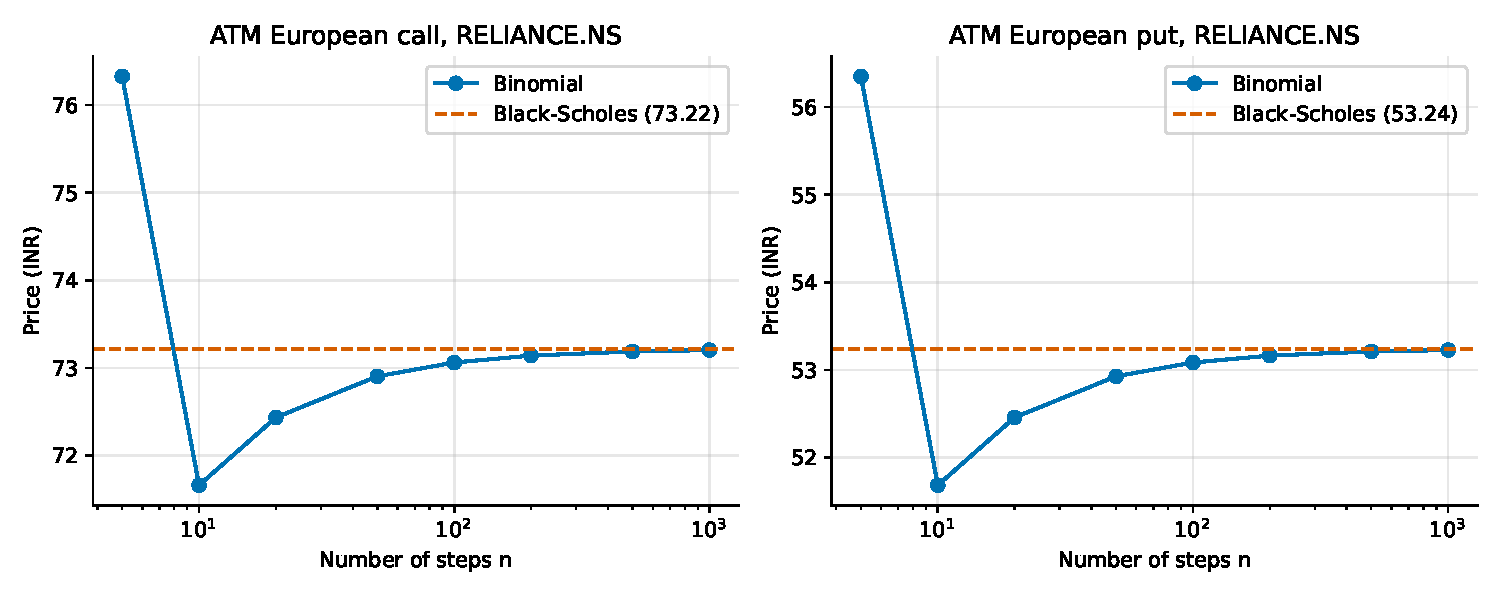
\includegraphics[width=\textwidth]{e1_convergence}
\caption{Binomial price against the number of steps $n$ (log axis), with the BS price as a dashed line. At-the-money European call (left) and put (right) on Reliance.}
\label{fig:e1}
\end{figure}

Each tenfold increase in $n$ reduces the error about tenfold. The absolute errors of the call and of the put are identical to the printed precision in Table~\ref{tab:e1_convergence}. This is expected: both models satisfy put--call parity, so $C^{\text{bin}} - C^{\text{BS}} = P^{\text{bin}} - P^{\text{BS}}$. Table~\ref{tab:e8_parity} confirms that the parity residuals are zero up to floating-point rounding.

\begin{table}
\centering
\small
\caption{Put-call parity residual $C-P-(S_0-Ke^{-rT})$.}
\label{tab:e8_parity}
\begin{adjustbox}{max width=\textwidth}
\begin{tabular}{lr}
\toprule
Model & Residual \\
\midrule
Black-Scholes & -1.13687e-13 \\
Binomial (n=500) & 1.80265e-11 \\
\bottomrule
\end{tabular}
\end{adjustbox}
\end{table}


\subsection{Rate of convergence and the odd/even oscillation}

The left panel of Figure~\ref{fig:e2} plots the absolute call error against $n$ for every $n$ from $5$ to $400$ on log--log axes. The points lie on a straight line of slope $-1$. Fitted separately, the slopes are $-1.00$ for odd $n$ and $-1.00$ for even $n$ (Table~\ref{tab:e2_slope}), so the error is $O(1/n)$. Numerically, $n \times \text{error} \approx 15.8$ INR for $n \geq 100$, i.e.\ about $0.016$ INR at $n = 1000$.

\begin{figure}[htbp]
\centering
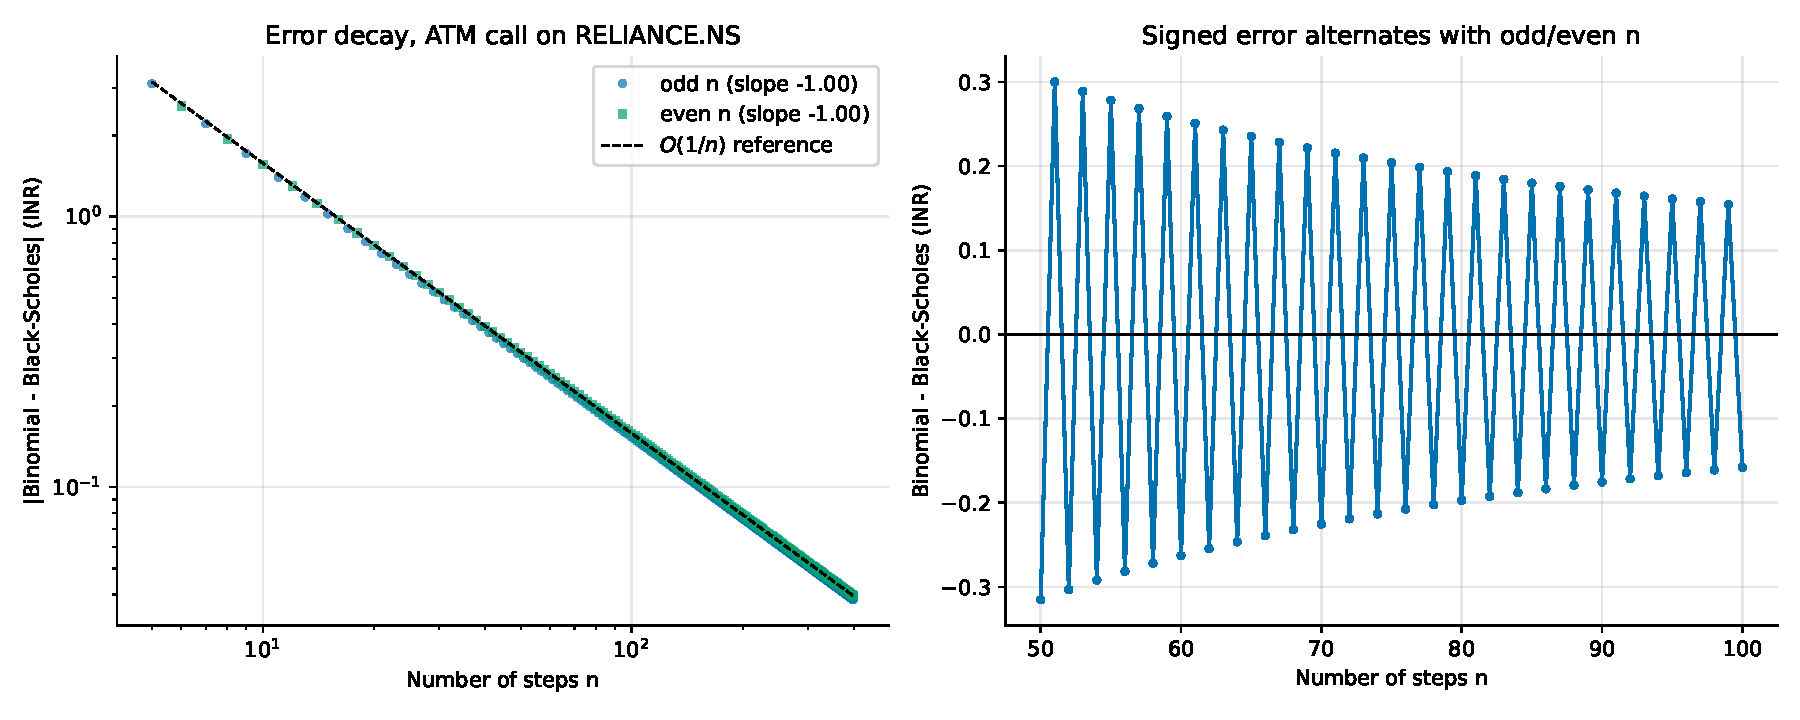
\includegraphics[width=\textwidth]{e2_error_loglog}
\caption{Left: absolute error of the at-the-money Reliance call against $n$, log--log, with an $O(1/n)$ reference line. Right: the signed error (binomial minus BS) for $n = 50,\dots,100$.}
\label{fig:e2}
\end{figure}

\begin{table}
\centering
\small
\caption{Fitted log-log slope of the absolute error against n (expected about $-1$).}
\label{tab:e2_slope}
\begin{adjustbox}{max width=\textwidth}
\begin{tabular}{lr}
\toprule
Subset & Fitted slope \\
\midrule
odd n & -1.00204 \\
even n & -0.997464 \\
\bottomrule
\end{tabular}
\end{adjustbox}
\end{table}


For this at-the-money strike the \emph{size} of the error is almost identical for odd and even $n$, so the two sets of points in the left panel coincide. The oscillation is in the \emph{sign}: the right panel shows the error alternating between about $-0.3$ and $+0.3$ INR at $n = 50$ and about $\mp 0.16$ INR at $n = 100$ from one value of $n$ to the next, negative for even $n$ and positive for odd $n$ in this range, so its envelope shrinks like $1/n$. (In Table~\ref{tab:e1_convergence} the binomial price is below BS for $n \geq 10$ only because those values of $n$ are even; $n = 5$ is odd and lies above.) For strikes away from the money, calculations for $K = 1.05\,S_0$ and $K = 1.1\,S_0$ show that the size of the error also depends on the parity of $n$. This is the well-known sawtooth behaviour of the CRR tree \cite{leisenreimer1996}; it is not a bug. It also means that the error at one particular $n$ is not a reliable guide to the error at $n \pm 1$.

\subsection{Effect of the strike}

Figure~\ref{fig:e3} and Table~\ref{tab:e3_strike} vary the strike from $0.8\,S_0$ to $1.2\,S_0$ at $n = 500$. The call price falls and the put price rises with the strike, and the two models agree closely everywhere: the largest absolute error in the table is $0.032$ INR, on a call worth $73.2$ INR. The error is not a smooth function of the strike. It is largest near the money ($0.032$ at $K = S_0$, $0.027$ at $1.05\,S_0$) but also $0.029$ at $1.15\,S_0$, and small ($0.001$) at $0.9\,S_0$. This irregular pattern comes from the position of the strike relative to the terminal lattice prices, the same mechanism as the odd/even oscillation.

\begin{table}
\centering
\small
\caption{Effect of strike (n=500, T=0.25) on RELIANCE.NS.}
\label{tab:e3_strike}
\begin{adjustbox}{max width=\textwidth}
\begin{tabular}{rrrrrrrr}
\toprule
K/S0 & K & BS call & Binomial call & Call abs err & BS put & Binomial put & Put abs err \\
\midrule
0.8 & 1056 & 281.224 & 281.222 & 0.00221182 & 1.24167 & 1.23945 & 0.00221182 \\
0.85 & 1122 & 219.421 & 219.415 & 0.00616354 & 4.44002 & 4.43386 & 0.00616354 \\
0.9 & 1188 & 162.299 & 162.3 & 0.0010957 & 12.3189 & 12.32 & 0.0010957 \\
0.95 & 1254 & 112.801 & 112.81 & 0.00955252 & 27.8221 & 27.8316 & 0.00955252 \\
1 & 1320 & 73.219 & 73.1874 & 0.0316032 & 53.2414 & 53.2098 & 0.0316032 \\
1.05 & 1386 & 44.2576 & 44.2848 & 0.0271882 & 89.2811 & 89.3083 & 0.0271882 \\
1.1 & 1452 & 24.9105 & 24.9001 & 0.0103845 & 134.935 & 134.925 & 0.0103845 \\
1.15 & 1518 & 13.0834 & 13.0544 & 0.029064 & 188.109 & 188.08 & 0.029064 \\
1.2 & 1584 & 6.43492 & 6.41274 & 0.0221733 & 246.462 & 246.44 & 0.0221733 \\
\bottomrule
\end{tabular}
\end{adjustbox}
\end{table}


\begin{figure}[htbp]
\centering
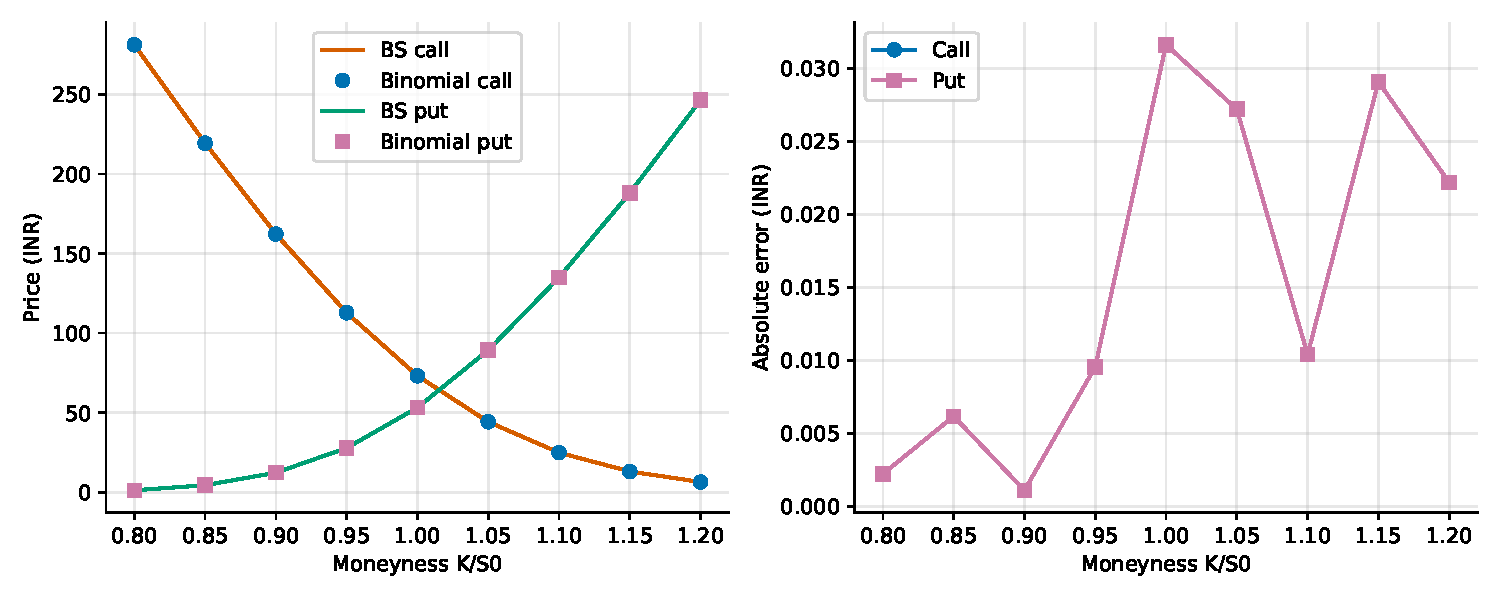
\includegraphics[width=\textwidth]{e3_strike}
\caption{Left: BS and binomial ($n = 500$) call and put prices against moneyness $K/S_0$, Reliance. Right: absolute error of the two.}
\label{fig:e3}
\end{figure}

\subsection{Effect of volatility}

Figure~\ref{fig:e4} and Table~\ref{tab:e4_volatility} vary $\sigma$ from $0.10$ to $0.60$ for the at-the-money option. Prices rise almost linearly with $\sigma$ (the call from $37.3$ to $166.4$ INR). The absolute error also grows with $\sigma$, from $0.014$ at $\sigma = 0.10$ to $0.078$ at $\sigma = 0.60$, which is roughly in proportion to the option price. Higher volatility makes each up and down move larger, so a tree with a given number of steps is coarser.

\begin{table}
\centering
\small
\caption{Effect of volatility (ATM, n=500, T=0.25) on RELIANCE.NS.}
\label{tab:e4_volatility}
\begin{adjustbox}{max width=\textwidth}
\begin{tabular}{rrrrrrr}
\toprule
sigma & BS call & Binomial call & Call abs err & BS put & Binomial put & Put abs err \\
\midrule
0.1 & 37.3227 & 37.3091 & 0.0136264 & 17.3451 & 17.3315 & 0.0136264 \\
0.15 & 49.983 & 49.963 & 0.0199803 & 30.0054 & 29.9854 & 0.0199803 \\
0.2 & 62.8347 & 62.8083 & 0.0264106 & 42.8571 & 42.8307 & 0.0264106 \\
0.25 & 75.7583 & 75.7254 & 0.0328728 & 55.7807 & 55.7478 & 0.0328728 \\
0.3 & 88.7119 & 88.6725 & 0.0393487 & 68.7342 & 68.6949 & 0.0393487 \\
0.35 & 101.676 & 101.63 & 0.0458294 & 81.6986 & 81.6528 & 0.0458294 \\
0.4 & 114.641 & 114.589 & 0.0523099 & 94.6632 & 94.6109 & 0.0523099 \\
0.45 & 127.599 & 127.54 & 0.0587869 & 107.621 & 107.562 & 0.0587869 \\
0.5 & 140.545 & 140.48 & 0.065258 & 120.568 & 120.502 & 0.065258 \\
0.55 & 153.476 & 153.405 & 0.071721 & 133.499 & 133.427 & 0.071721 \\
0.6 & 166.389 & 166.311 & 0.0781746 & 146.411 & 146.333 & 0.0781746 \\
\bottomrule
\end{tabular}
\end{adjustbox}
\end{table}


\begin{figure}[htbp]
\centering
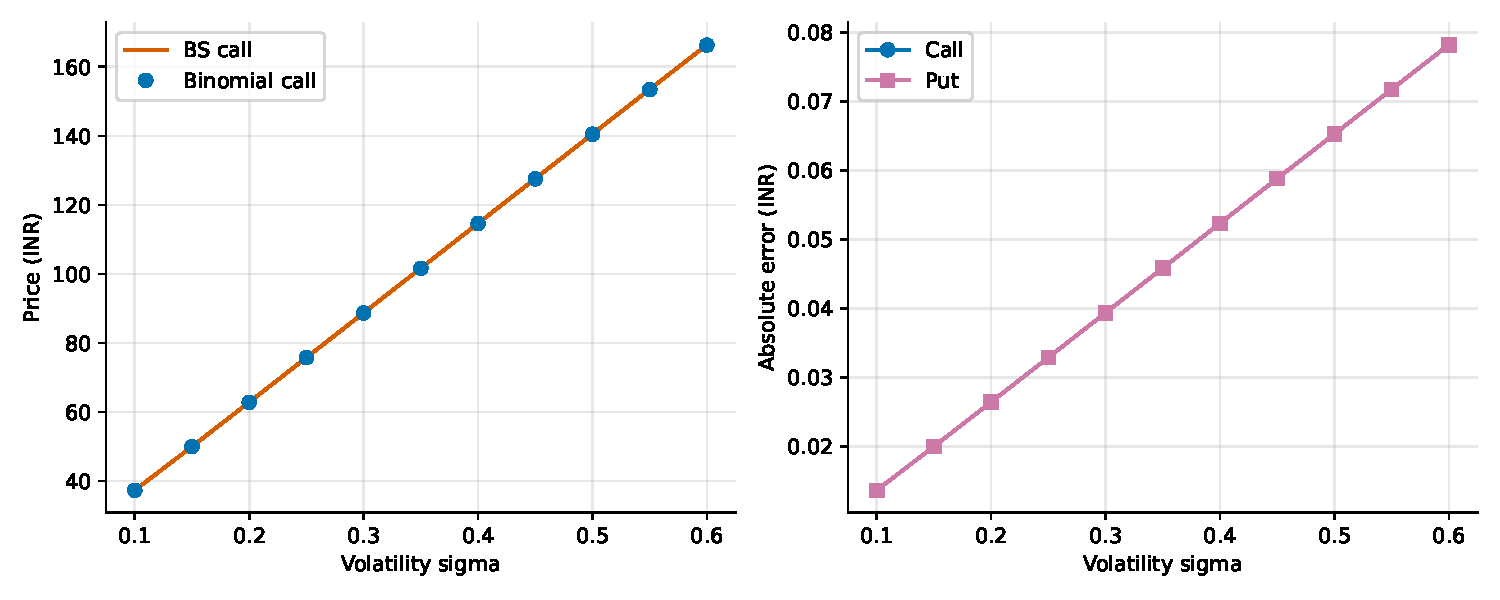
\includegraphics[width=\textwidth]{e4_volatility}
\caption{Left: BS and binomial call price against volatility $\sigma$ (at the money, $n = 500$). Right: absolute error of the call and put.}
\label{fig:e4}
\end{figure}

\subsection{Effect of maturity}

Figure~\ref{fig:e5} and Table~\ref{tab:e5_maturity} vary $T$ from one month to one year. Option prices increase with maturity, and so does the absolute error at fixed $n$: it rises from $0.018$ INR at one month to $0.063$ INR at one year. The ratio of these errors, about $3.5$, is close to $\sqrt{12} \approx 3.46$, the square root of the ratio of the maturities. This agrees with the fact that an at-the-money option price grows like $\sigma\sqrt{T}$, and that the error is proportional to the price at a fixed $n$. Longer maturity at fixed $n$ also means a larger step $\Delta t$.

\begin{table}
\centering
\small
\caption{Effect of maturity (ATM, n=500) on RELIANCE.NS.}
\label{tab:e5_maturity}
\begin{adjustbox}{max width=\textwidth}
\begin{tabular}{rrrrrrr}
\toprule
T (years) & BS call & Binomial call & Call abs err & BS put & Binomial put & Put abs err \\
\midrule
0.0833333 & 39.8572 & 39.839 & 0.0182505 & 33.1642 & 33.1459 & 0.0182505 \\
0.25 & 73.219 & 73.1874 & 0.0316032 & 53.2414 & 53.2098 & 0.0316032 \\
0.5 & 109.227 & 109.182 & 0.0446668 & 69.5736 & 69.529 & 0.0446668 \\
1 & 165.412 & 165.349 & 0.0630399 & 87.2973 & 87.2343 & 0.0630399 \\
\bottomrule
\end{tabular}
\end{adjustbox}
\end{table}


\begin{figure}[htbp]
\centering
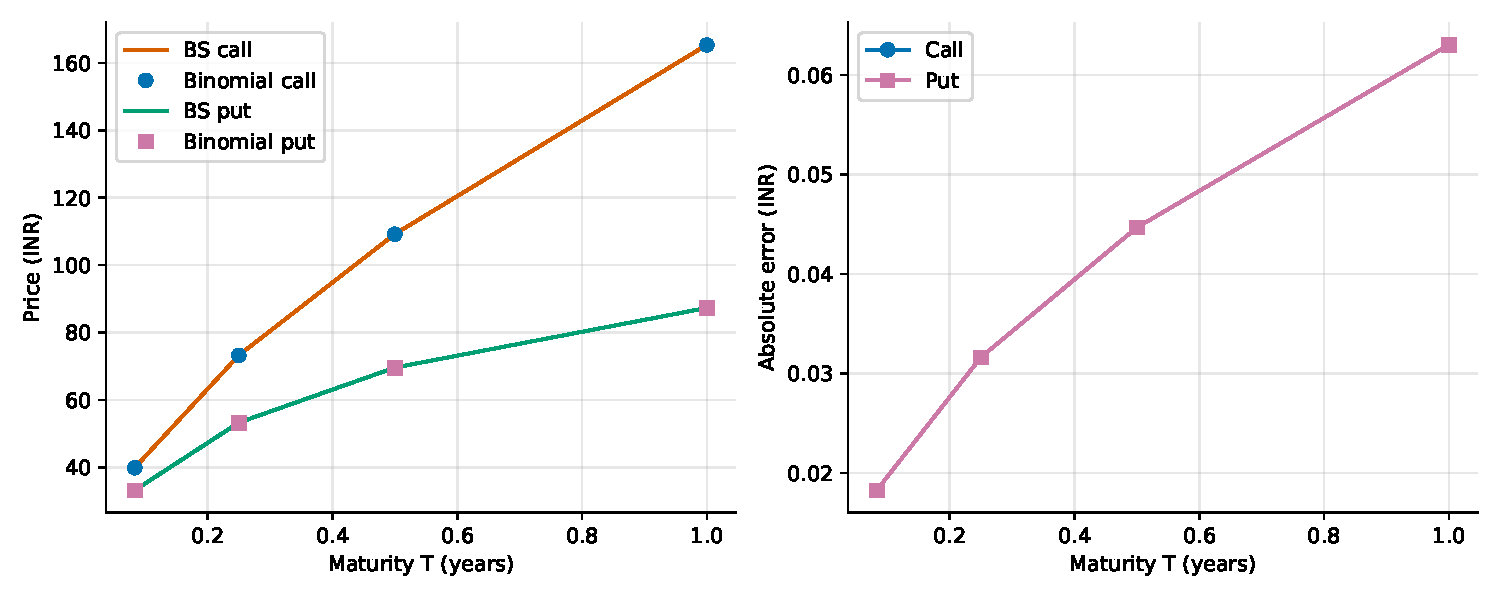
\includegraphics[width=\textwidth]{e5_maturity}
\caption{Left: BS and binomial prices against maturity $T$ (at the money, $n = 500$). Right: absolute error.}
\label{fig:e5}
\end{figure}

\subsection{Comparison across stocks}

Table~\ref{tab:e6_stocks} and Figure~\ref{fig:e6} price the at-the-money three-month options on each stock with its own $S_0$ and $\hat\sigma$.

\begin{table}
\centering
\small
\caption{Same moneyness (ATM), T=0.25, n=500, for each stock's own S0 and sigma.}
\label{tab:e6_stocks}
\begin{adjustbox}{max width=\textwidth}
\begin{tabular}{lrrrrrrrrrr}
\toprule
Stock & S0 & sigma & BS call & Binomial call & Call abs err & Call rel err & BS put & Binomial put & Put abs err & Put rel err \\
\midrule
RELIANCE.NS & 1320 & 0.240188 & 73.219 & 73.1874 & 0.0316032 & 0.000431626 & 53.2414 & 53.2098 & 0.0316032 & 0.000593584 \\
SUNPHARMA.NS & 1860 & 0.195901 & 87.0503 & 87.0138 & 0.03647 & 0.000418953 & 58.9 & 58.8635 & 0.03647 & 0.000619185 \\
ADANIENT.NS & 2745.8 & 0.37479 & 224.874 & 224.772 & 0.102016 & 0.00045366 & 183.317 & 183.215 & 0.102016 & 0.000556501 \\
\bottomrule
\end{tabular}
\end{adjustbox}
\end{table}


\begin{figure}[htbp]
\centering
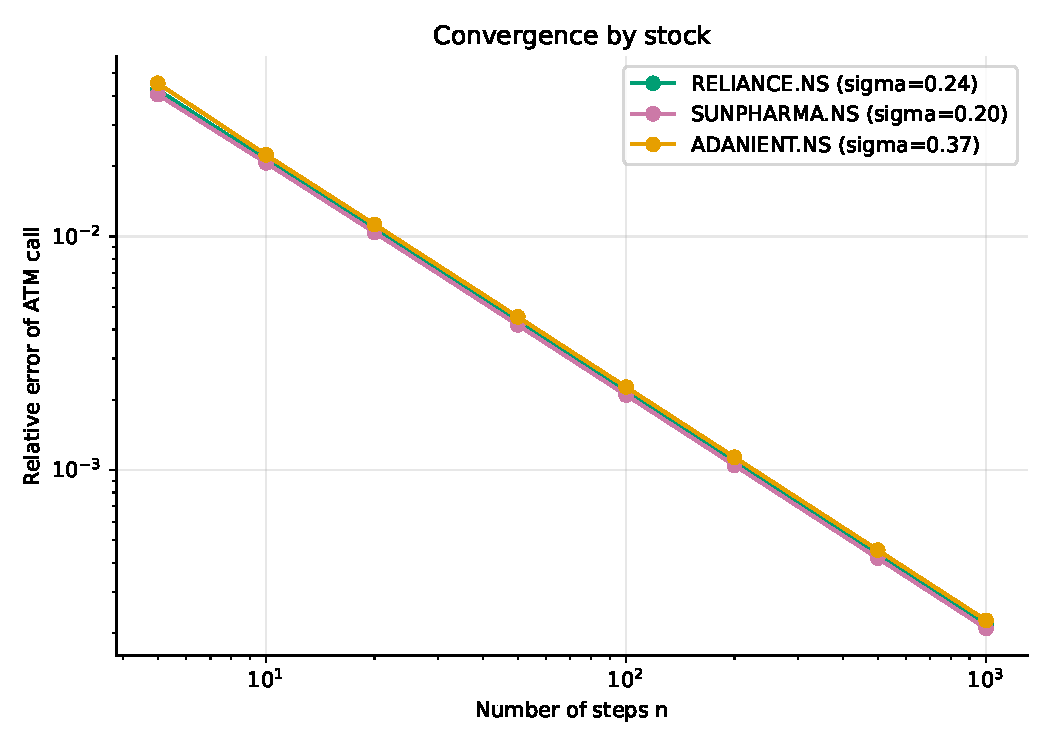
\includegraphics[width=0.75\textwidth]{e6_stocks_convergence}
\caption{Relative error of the at-the-money call against $n$ for each stock (log--log). The three curves nearly coincide.}
\label{fig:e6}
\end{figure}

The absolute errors differ greatly (from $0.032$ INR for Reliance to $0.102$ INR for Adani Enterprises at $n = 500$) because the stocks have different prices and volatilities. The \emph{relative} errors are much closer. For the call they are $4.19\times10^{-4}$ (Sun Pharma, $\hat\sigma = 0.196$), $4.32\times10^{-4}$ (Reliance, $0.240$) and $4.54\times10^{-4}$ (Adani, $0.375$): they rise slightly with volatility, but the highest value is only about $8\%$ above the lowest even though $\hat\sigma$ almost doubles. For the put the relative errors are $6.19\times10^{-4}$, $5.94\times10^{-4}$ and $5.57\times10^{-4}$ and move in the opposite direction, because a put is relatively more expensive at higher volatility while its error is identical to the call's. In both cases the convergence curves in Figure~\ref{fig:e6} are almost on top of one another. Within this set of stocks, convergence is essentially governed by $n$, not by which company is priced.

\subsection{Running time}

Table~\ref{tab:e7_timing} and Figure~\ref{fig:e7} report the median time to compute one price (the BS function, and the binomial function at each $n$) on the project machine.

\begin{table}
\centering
\small
\caption{Median running time per option price.}
\label{tab:e7_timing}
\begin{adjustbox}{max width=\textwidth}
\begin{tabular}{lrr}
\toprule
Method & n & Seconds per price \\
\midrule
Black-Scholes & 0 & 6.82618e-05 \\
Binomial & 5 & 1.53257e-05 \\
Binomial & 10 & 2.41351e-05 \\
Binomial & 20 & 4.13792e-05 \\
Binomial & 50 & 9.2669e-05 \\
Binomial & 100 & 0.000182422 \\
Binomial & 200 & 0.000387456 \\
Binomial & 500 & 0.00102853 \\
Binomial & 1000 & 0.00232483 \\
\bottomrule
\end{tabular}
\end{adjustbox}
\end{table}


\begin{figure}[htbp]
\centering
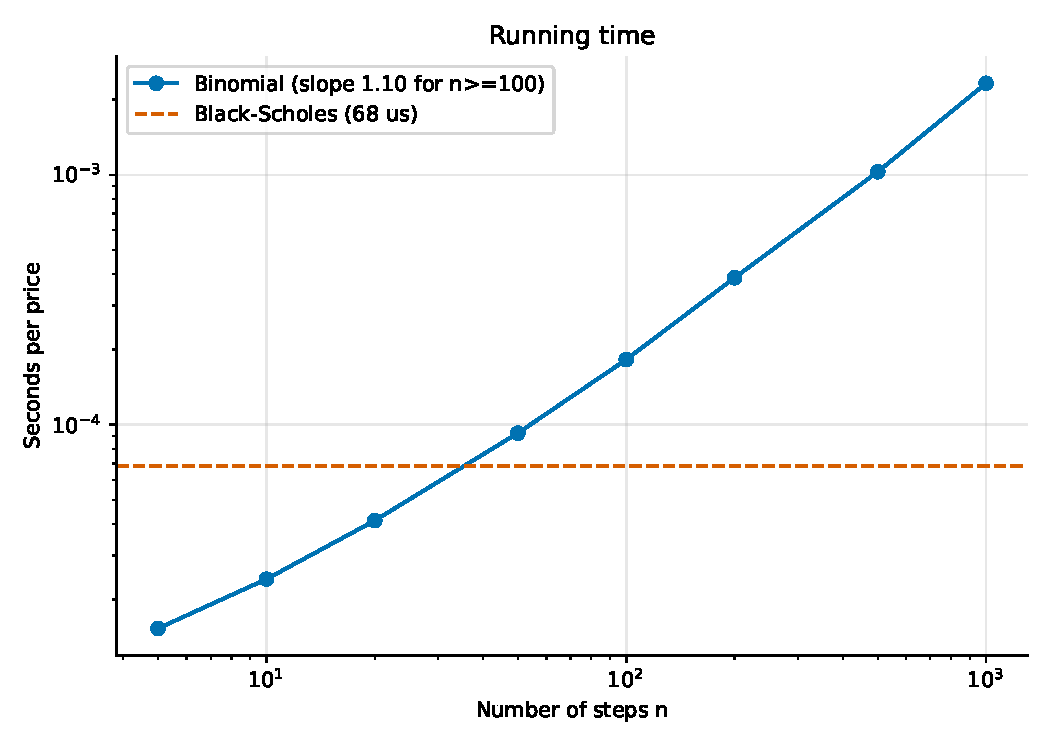
\includegraphics[width=0.75\textwidth]{e7_timing}
\caption{Median time per price against $n$ (log--log). The dashed line is the BS time, which does not depend on $n$.}
\label{fig:e7}
\end{figure}

The BS formula takes about $70\ \mu$s per price, independent of $n$. The binomial price takes about $15\ \mu$s at $n = 5$ (faster than BS in our implementation, because the SciPy normal-distribution call has a fixed overhead), $0.18$ ms at $n = 100$, $1.0$ ms at $n = 500$ and $2.3$ ms at $n = 1000$, about $34$ times the BS time. Theoretically the work grows like $n^2$, but the fitted log--log slope for $n \geq 100$ is only about $1.1$ (Table~\ref{tab:e7_slope}). Each of the $n$ steps is a single vectorised NumPy operation on at most $n+1$ numbers, so for $n \leq 1000$ the fixed cost per Python loop iteration dominates and the cost looks nearly linear. To check this we extended the sweep to $n = 16{,}000$ in a separate run (\texttt{extensions.py}, Table~\ref{tab:e10_timing_large_n}): for $n \geq 4000$ the fitted slope is about $2.1$ (Table~\ref{tab:e10_slope}), so once the arithmetic outweighs the fixed cost per step the running time grows like $n^2$, as expected.

\begin{table}
\centering
\small
\caption{Median running time per binomial price for large n.}
\label{tab:e10_timing_large_n}
\begin{adjustbox}{max width=\textwidth}
\begin{tabular}{rr}
\toprule
n & Seconds per price \\
\midrule
1000 & 0.00705337 \\
2000 & 0.0101596 \\
4000 & 0.0276605 \\
8000 & 0.110355 \\
16000 & 0.517321 \\
\bottomrule
\end{tabular}
\end{adjustbox}
\end{table}

\begin{table}
\centering
\small
\caption{Log-log slope of binomial running time against n, large n.}
\label{tab:e10_slope}
\begin{adjustbox}{max width=\textwidth}
\begin{tabular}{r}
\toprule
Fitted slope (n >= 4000) \\
\midrule
2.11258 \\
\bottomrule
\end{tabular}
\end{adjustbox}
\end{table}


\begin{table}
\centering
\small
\caption{Log-log slope of binomial running time against n.}
\label{tab:e7_slope}
\begin{adjustbox}{max width=\textwidth}
\begin{tabular}{r}
\toprule
Fitted slope (n >= 100) \\
\midrule
1.09987 \\
\bottomrule
\end{tabular}
\end{adjustbox}
\end{table}


%% ------------------------------------------------------------------
\section{Discussion}\label{sec:discussion}

\textbf{Accuracy.} Everything measured here is consistent with the CRR tree converging to Black--Scholes at first order. With $n = 500$ the relative error of an at-the-money call is about $0.04\%$ for all three stocks; to halve the error one must double $n$, which roughly doubles the work in our implementation and quadruples it asymptotically.

\textbf{Oscillation and the choice of $n$.} Because the error changes sign with the parity of $n$, a single binomial price can be above or below the BS price by a similar amount. Averaging the prices for $n$ and $n+1$ cancels most of it (Table~\ref{tab:e9_averaging}, Figure~\ref{fig:e9}). For the at-the-money Reliance call the error falls from $0.158$ to $0.0033$ INR at $n = 100$ (48 times smaller) and from $0.0316$ to $0.00056$ INR at $n = 500$ (56 times smaller). The average costs about two trees, but it still beats a single tree of twice the size: $0.0033$ INR against $0.079$ INR for $n = 200$. Away from the money the gain is smaller and irregular: at $n = 500$ the error falls 14 times for $K = 1.05\,S_0$ and 4 times for $K = 1.1\,S_0$, but at $n = 200$ for $K = 1.05\,S_0$ and at $n = 50$ for $K = 1.1\,S_0$ the average is worse than the plain tree, which happens to be almost exact there. Averaging removes the odd/even alternation, but not the part of the error that comes from where the strike sits between two terminal nodes.

\begin{table}
\centering
\small
\caption{Call error of one tree (n and 2n steps) and of the average of n and n+1 steps, RELIANCE.NS, T=0.25.}
\label{tab:e9_averaging}
\begin{adjustbox}{max width=\textwidth}
\begin{tabular}{rrrrrr}
\toprule
K/S0 & n & Plain err (n) & Plain err (2n) & Averaged err (n, n+1) & Plain / averaged \\
\midrule
1 & 10 & 1.55843 & 0.785036 & 0.0785975 & 19.8279 \\
1 & 50 & 0.315302 & 0.157856 & 0.00762858 & 41.3316 \\
1 & 100 & 0.157856 & 0.0789782 & 0.00325889 & 48.4384 \\
1 & 200 & 0.0789782 & 0.0395015 & 0.00148845 & 53.0606 \\
1 & 500 & 0.0316032 & 0.0158036 & 0.000561266 & 56.3071 \\
1 & 1000 & 0.0158036 & 0.00790229 & 0.000274924 & 57.4835 \\
1.05 & 10 & 1.18871 & 0.324643 & 0.596941 & 1.99134 \\
1.05 & 50 & 0.26469 & 0.133984 & 0.0229467 & 11.535 \\
1.05 & 100 & 0.133984 & 0.0161766 & 0.000563143 & 237.922 \\
1.05 & 200 & 0.0161766 & 0.0247232 & 0.0215769 & 0.749719 \\
1.05 & 500 & 0.0271882 & 0.0130427 & 0.0019943 & 13.633 \\
1.05 & 1000 & 0.0130427 & 0.00378737 & 0.00219151 & 5.95146 \\
1.1 & 10 & 0.17379 & 0.117764 & 0.0891769 & 1.94883 \\
1.1 & 50 & 0.00127967 & 0.136639 & 0.0587779 & 0.0217714 \\
1.1 & 100 & 0.136639 & 0.0407585 & 0.0224595 & 6.08381 \\
1.1 & 200 & 0.0407585 & 0.0265802 & 0.00613191 & 6.64695 \\
1.1 & 500 & 0.0103845 & 0.00907207 & 0.00249346 & 4.16469 \\
1.1 & 1000 & 0.00907207 & 0.00150277 & 0.00128786 & 7.04428 \\
\bottomrule
\end{tabular}
\end{adjustbox}
\end{table}


\begin{figure}[htbp]
\centering
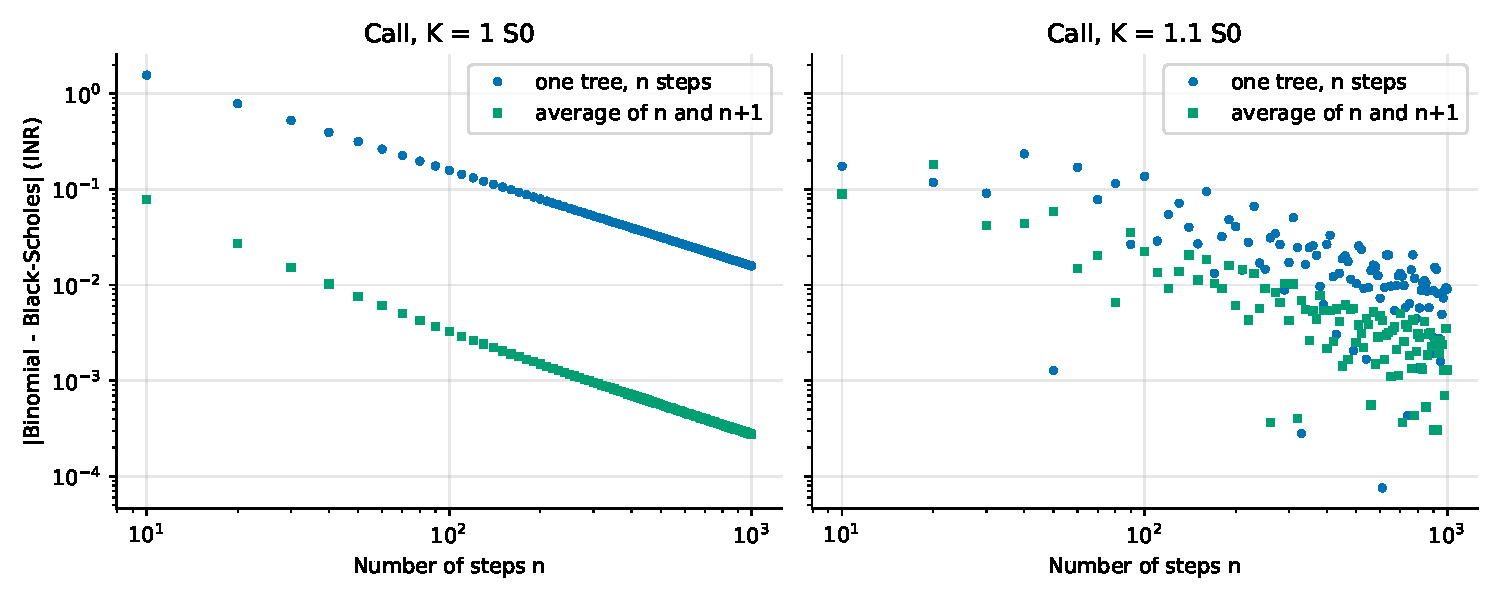
\includegraphics[width=\textwidth]{e9_averaging}
\caption{Absolute call error of one tree with $n$ steps and of the average of the $n$- and $(n+1)$-step prices, Reliance, at the money (left) and $K = 1.1\,S_0$ (right).}
\label{fig:e9}
\end{figure}

\textbf{Sensitivity to the inputs.} The qualitative behaviour of both models is the same and is the one expected from option theory: call prices fall and put prices rise with the strike, and both prices rise with volatility and maturity. The binomial error grows with $\sigma$ and with $\sqrt{T}$ at fixed $n$, roughly in proportion to the option price, and depends irregularly on the strike.

\textbf{Speed versus flexibility.} For European options under constant $\sigma$ and $r$ the Black--Scholes formula is both exact (within the model) and about $34$ times cheaper than a $1000$-step tree, so the tree has no advantage on this problem. The tree's attraction is that the backward induction \eqref{eq:backward} can be modified at each node, for example to allow early exercise or discrete dividends, where no closed form exists.

\textbf{What ``error'' means here.} The BS price is used as the reference because it is the exact price under the GBM assumption. The error we report is therefore the discretisation error of the tree, not the error of either model against actual market option prices, which we did not use.

%% ------------------------------------------------------------------
\section{Limitations}\label{sec:limitations}

\begin{itemize}
  \item \textbf{Constant volatility and rate.} Both models assume that $\sigma$ and $r$ are constant over the option's life. The rate is a fixed input (default $6.29\%$, overridable with \texttt{--rate}) rather than an automatically fetched current value, and it is not matched to each option's maturity (see Section~\ref{sec:data}). Real volatility changes over time, and Adani Enterprises in particular has shocks driven by news that GBM does not capture.
  \item \textbf{Historical volatility.} $\hat\sigma$ is estimated from one year of past prices. It depends on the window used, and is not the volatility implied by market option prices.
  \item \textbf{Log-normal returns.} GBM implies thin tails; real returns have fatter tails and jumps.
  \item \textbf{European exercise only.} We priced neither American options nor options on dividend-paying stocks explicitly (dividends enter only through the adjusted price history).
  \item \textbf{No market comparison.} We compare two models with each other; no observed option prices were used.
  \item \textbf{One date, three stocks.} All results use data up to 6 November 2026 for three stocks, and timing results depend on the machine and implementation.
\end{itemize}

%% ------------------------------------------------------------------
\section{Conclusion}\label{sec:conclusion}

We implemented the Black--Scholes formula and the Cox--Ross--Rubinstein binomial tree and used them to price European calls and puts on Reliance, Sun Pharma and Adani Enterprises, with volatility estimated from one year of daily prices and the RBI 364-day T-bill rate as the risk-free rate. The main findings are:
\begin{enumerate}
  \item The binomial price converges to the Black--Scholes price as $n$ grows, with error $O(1/n)$ (fitted log--log slope $-1.00$). For an at-the-money Reliance call the relative error is $0.22\%$ at $n = 100$ and $0.022\%$ at $n = 1000$.
  \item The error alternates in sign between odd and even $n$, and for strikes away from the money its size also depends on the parity of $n$.
  \item The call--put error is identical, and put--call parity holds in both models to rounding error.
  \item At fixed $n$ the absolute error grows with volatility and with maturity (like $\sqrt{T}$), and depends irregularly on the strike. Across the three stocks the relative error differs by less than $12\%$ although $\hat\sigma$ ranges from $0.196$ to $0.375$, so convergence is governed mainly by $n$ rather than by the company.
  \item Black--Scholes costs about $70\ \mu$s per price regardless of accuracy, whereas the tree needs about $2.3$ ms for $n = 1000$; for plain European options the formula is therefore faster and exact, and the tree is useful mainly as a base for extensions the formula cannot handle.
\end{enumerate}

\textbf{Reproducibility.} All figures and tables are regenerated by running \texttt{python compare.py} and then \texttt{python extensions.py} (Experiments E9 and E10, on the same inputs) in the project folder (add \texttt{--rate PERCENT} to use a different risk-free yield); the data used are recorded in \texttt{outputs/run\_info.json}.

\bibliographystyle{plain}
\bibliography{refs}

\end{document}
